
\subsection{Pneumatikzylinder}
\begin{figure}[h!]
	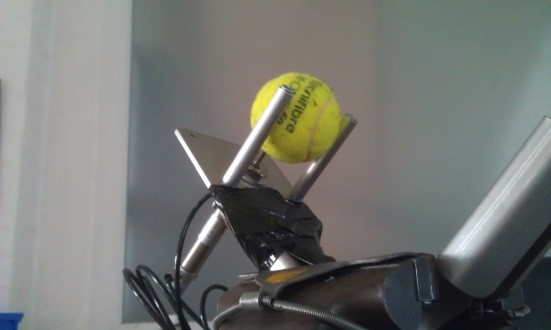
\includegraphics[width=5cm]{Funktionstests/Bilder/PneumatikzylinderBild.jpg}
	\centering
	\caption{Funktionsmuster Pneumatikzylinder} 
\label{abb:PneumatikzylinderBild}
\end{figure}	
\textit{Typ}: Pneumatikzylinder \\ 
\textit{Datum}: 8.10.2014   \\
\textit{Ort}: Bachmann Engineering AG (Zofingen) \\
\textit{Tester}: Gruppe 32 \\
\textit{Ziel des Testes}:  Das Ziel dieses Testes bestand darin, den gebauten Prototyp auf die Wurfwiederholgenauigkeit zu testen. \\
\textit{Fazit/ Verbesserungsvorschlag}: \\
Ein Pneumatikzylinder arbeitet sehr zielgenau und schnell.\\
Zu verbessern:\\
Es wurde ein überdimensionierter Zylinder für die Testzwecke verwendet. \\
benötigte Abschussgeschwindigkeit mittels schiefer Wurf bestimmen. Anschliessend mittels Stoss die 
benötigte Beschleunigung des Zylinders bestimmen und im Anschluss den Zylinder gemäss
ausgerechneten Daten (Druckversorgung / Kolbendurchmesser / Drosselung) ausglegen.\\
Mit einem kleineren kann an Gewicht und Kosten gespart werden. Als Ansteuerung reicht ein federrückgestelltes Magnetventil. \\
\textit{Ziel erreicht}: Ja